\documentclass{article}

\usepackage{stix2}
\usepackage{amsmath}\usepackage{amssymb}\usepackage{amsfonts}
\DeclareMathOperator{\s}{\mathscr{s}}

\usepackage[a4paper]{geometry}
\usepackage{siunitx}
\usepackage{circuitikz}\usepackage{pgfplots}
\usepackage{float}
\usepackage{subcaption}

\usetikzlibrary{pgfplots.smithchart}

\title{ECE218A --- Lab 01A}
\author{George Higgins Hutchinson \& Shouyan Li}

\begin{document}
\maketitle

\section{Introduction}

In this lab assignment, we used a Keysight E5063A ENA Network Analyzer to do several transmission line measurements and measure several important properties for passive devices. Afterwards, we simulated the transmission line and devices in ADS to make further comparison and analysis.

\section{Methods}

\subsection{Calibration}

To accomplish the lab, we stated with calibrating the network analyzer. The calibration process is critical to making accurate measurements because it can eliminate the errors and move the reference plane from the ports to the end tip of the cables. For this lab, we used the 85033E calibration kit, which later turned out to be defective and caused noisy and data in the measurements. The materials we used includes Duriod board (H=1.57048mm, L=14cm, $\epsilon_{r}=2.3 $), 5mm and 10mm Copper tape, and connectors and mounting blocks.


\begin{figure}[h]
    \centering
    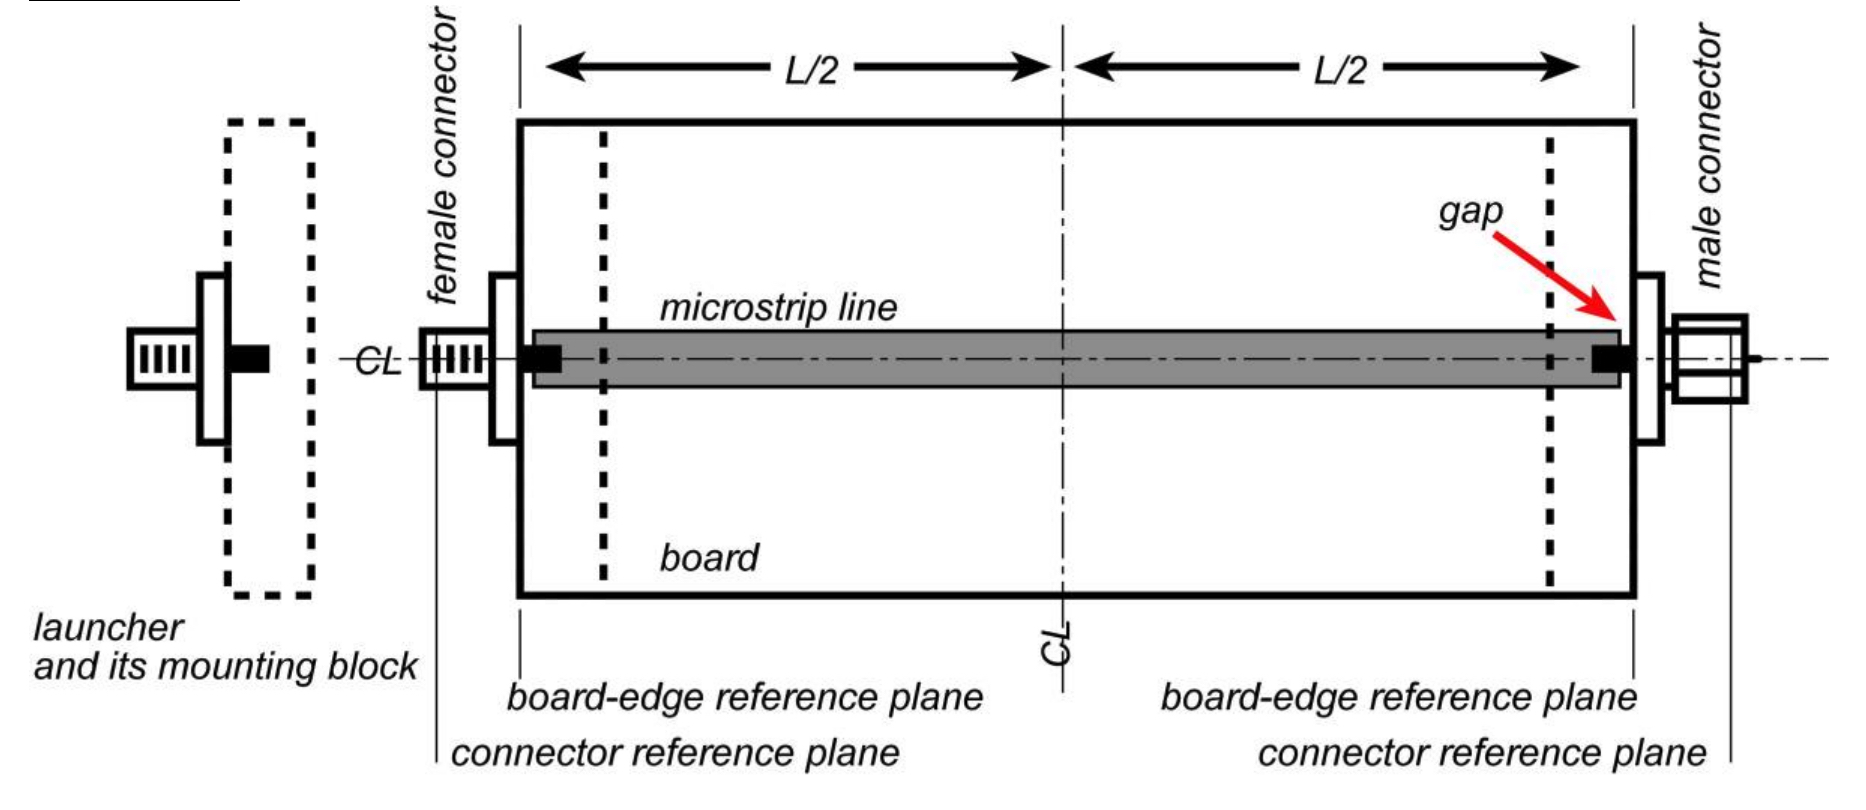
\includegraphics[width=0.8\textwidth]{figures/Short.jpg}
    \caption{Build mechanics for transmission line measurement}
\end{figure}

\begin{flushleft}
In order to get more accurate data, it is also necessary to move the reference from the connector reference plane to the board-edge reference plane(As Fig.1 shown above). To achieve this target, we built the board in a different way as the Figure 2 below illustrates.
\end{flushleft}

\begin{flushleft}
As the figure demonstrates, we short the line at both end. Therefore, after we connect the cable to the connector , we can tune the electrical delay to adjust the smith chart for $S_{11}$ and $S_{22}$ so that the graphs looks like short circuit. The electrical delay is later put into Scale-Electrical delay in the Network Analyzer. 
\end{flushleft}


\begin{figure}[h]
    \centering
    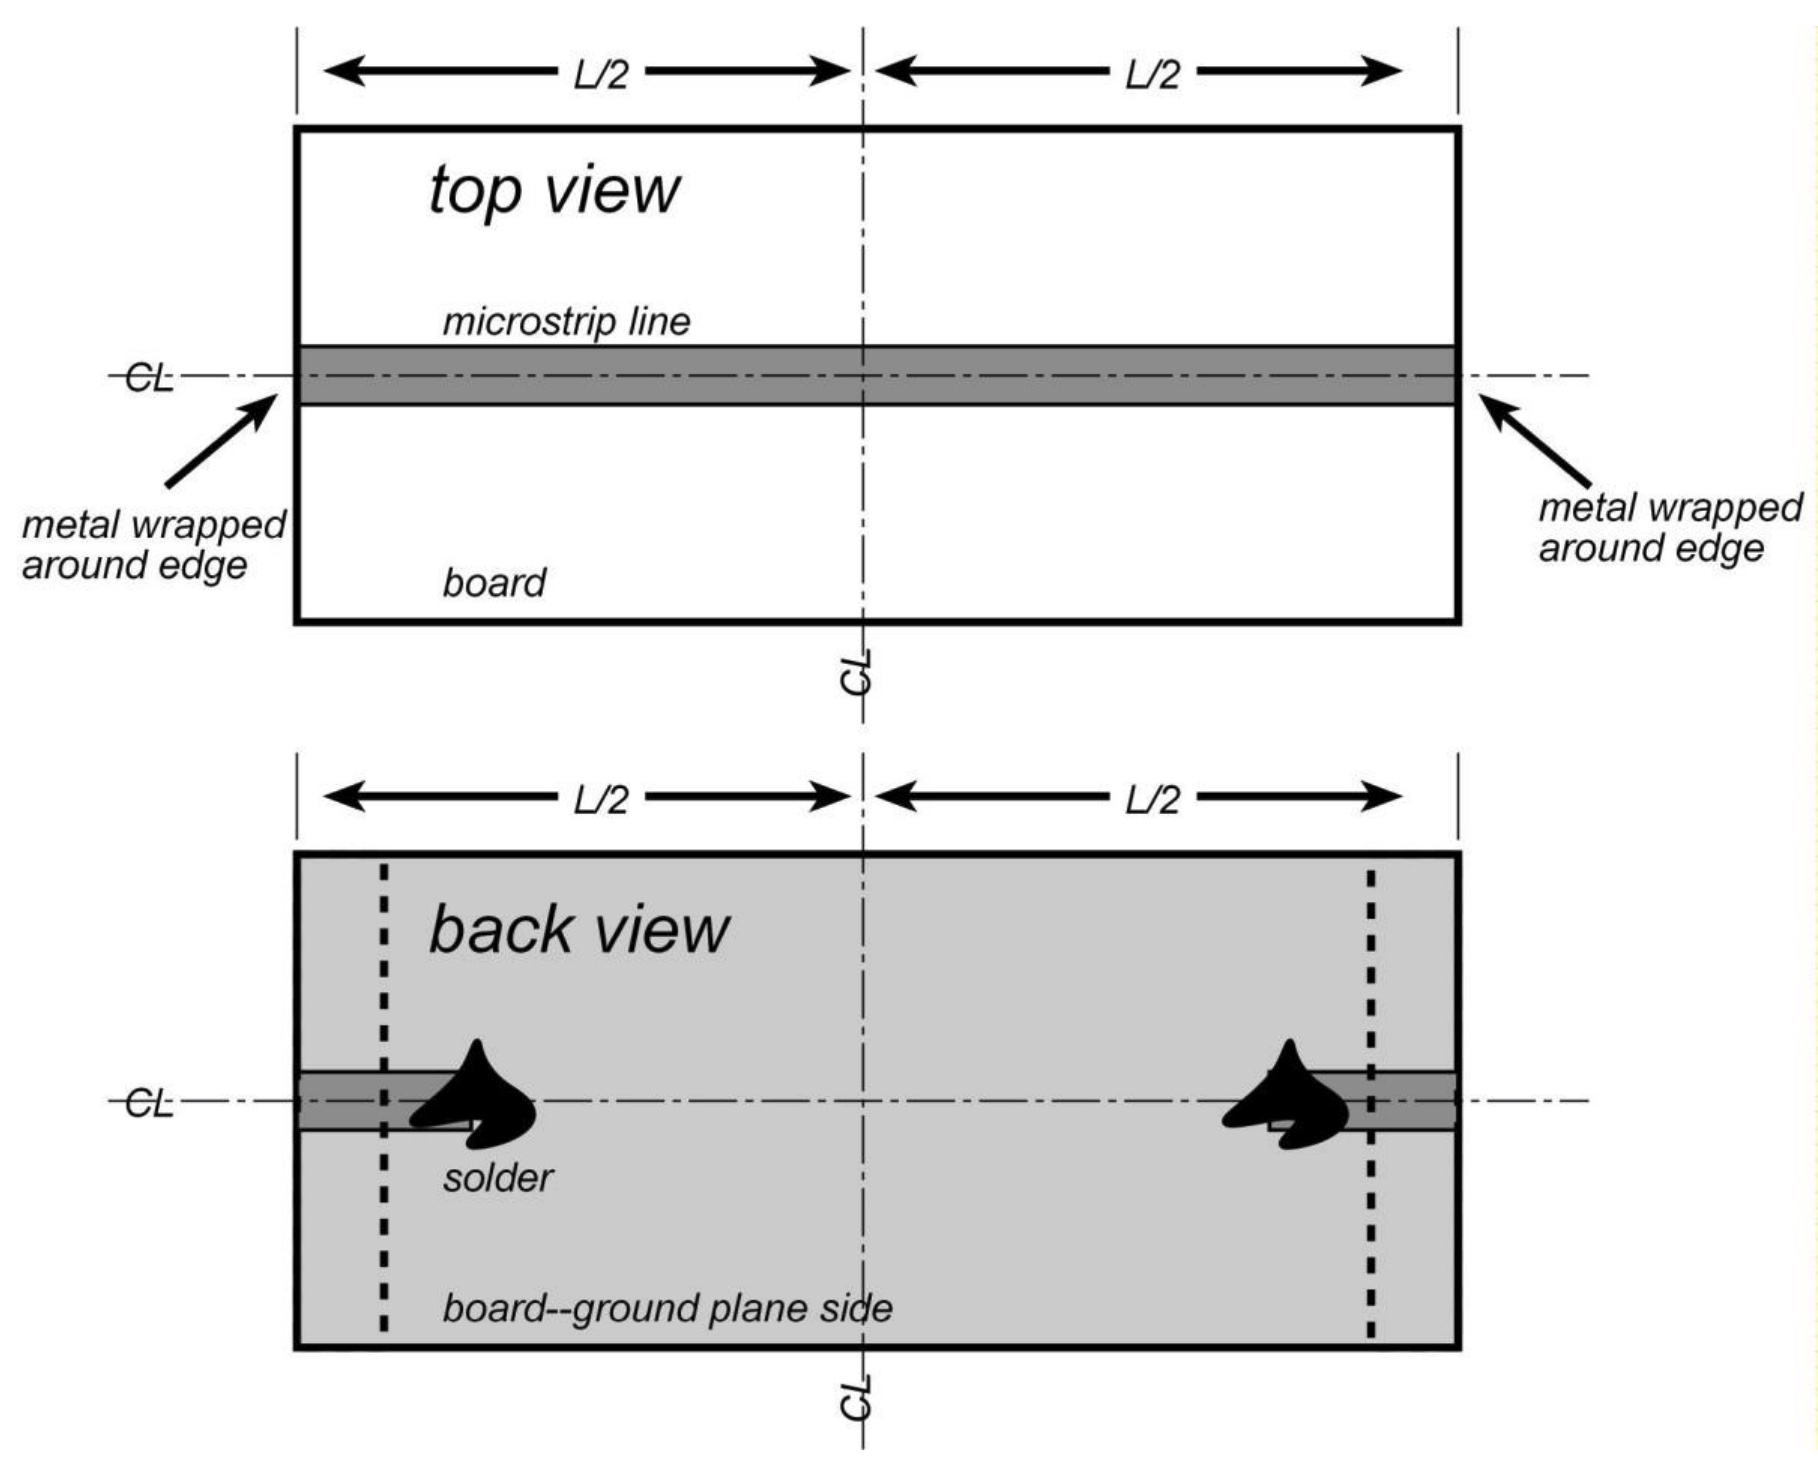
\includegraphics[width = 0.8\textwidth]{figures/connector.jpg}
    \caption{Build mechanics for reference plane extension}
\end{figure}




\subsection{Transmission Line Measurement}


\begin{flushleft}
The transmission line measurement includes two parts: the measurement of real physics device and simulation in the ADS software. We fabricated the device as Figure 1 shown in the previous sector. The only difference is that we used two female connectors instead due to the calibration kit limitation. We measured 3mm 5mm and 10mm copper tape respectively, and peeled of the tape to change the tape after each measurements. 

\end{flushleft}

\begin{flushleft}
To do the simulation, we first typed in the proprieties for the Duriod board into the LineCalc (Figure 4) to calculate theoretic characteristic impedance and shift, then imported the proprieties to the transmission line model in the ADS schematic as shown below. Finally, we adjusts the shift to make the simulation looks like the measurements. The results for the measurements and data will be analyzed in the result section below.
\end{flushleft}

\begin{figure}[H]
    \centering
    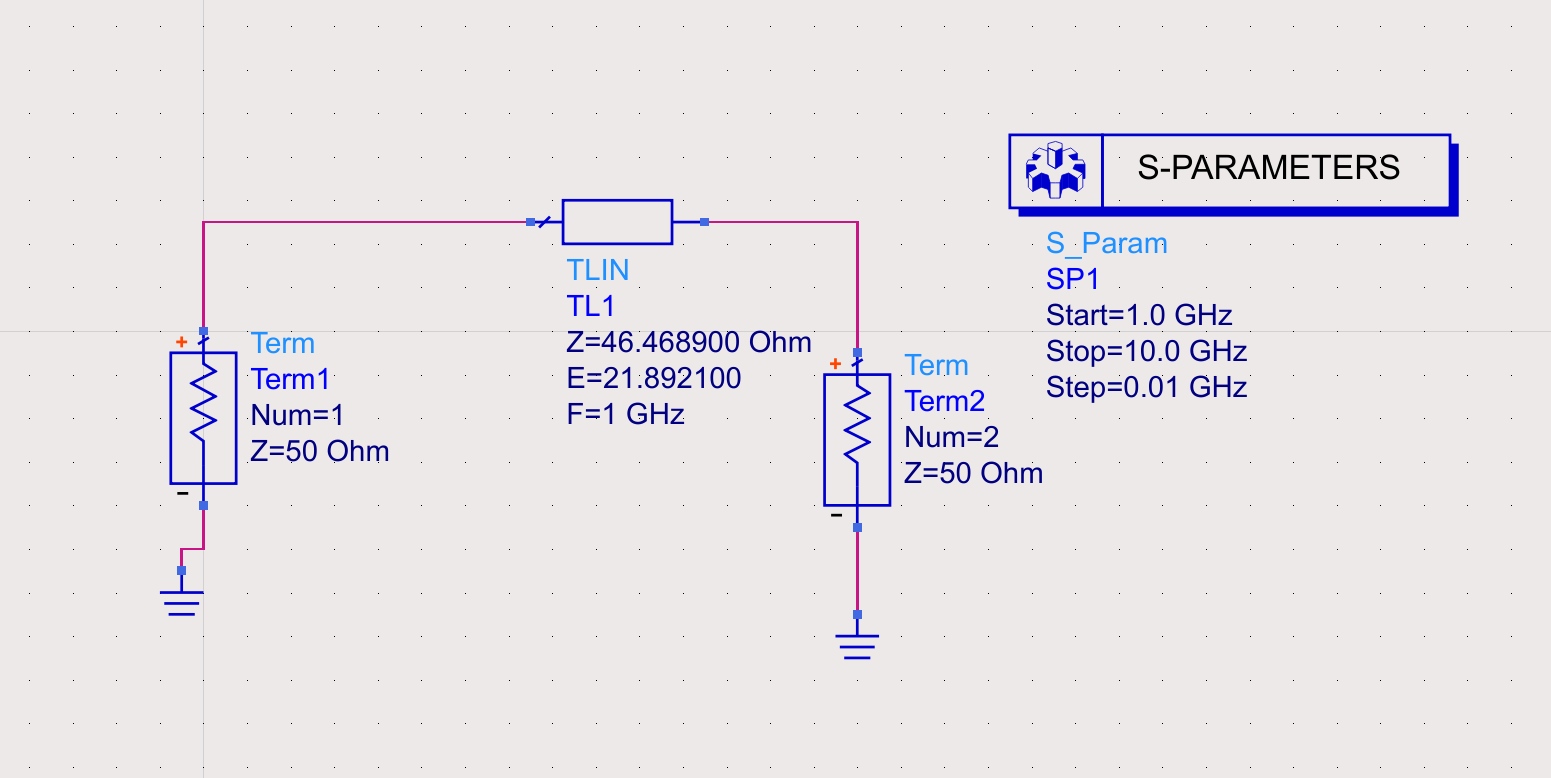
\includegraphics[width = 0.8\linewidth]{figures/schematic.PNG}
    \caption{Transmission Line Simulation Schematic}
\end{figure}

\begin{figure}[H]
    \centering
    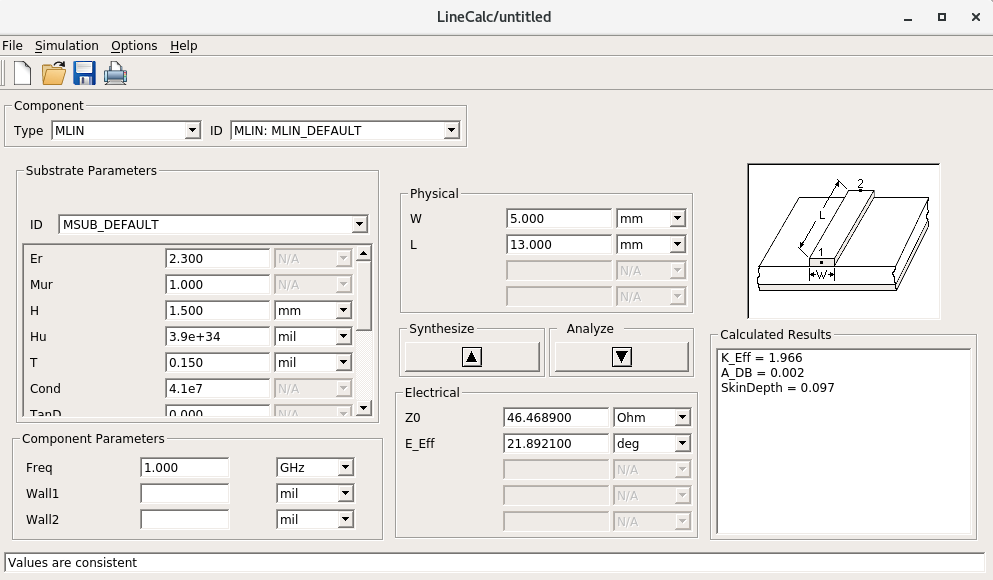
\includegraphics[width = 0.8\linewidth]{figures/linecalc.png}
    \caption{Transmission Line Simulation Schematic}
\end{figure}

\subsection{Passive Devices Measurement}

\begin{flushleft}

Finally, we conducted several measurements for the Passive Devices. The 
fabrication setup and and the simulation schematic are illustrated below. The passive devices include a 50 $\Omega$ 1/4-inch-long-leaded resistor a 50$\Omega$ very-short-leaded resistor, a 15 $\Omega$ chip resistor, a 100pF leaded capacitor, a 100pF chip capacitor, and a 30pH hand-made inductor.  The results for the measurements and simulation will also be analyzed and compared afterwards.
\end{flushleft}

\begin{figure}[H]
    \centering
    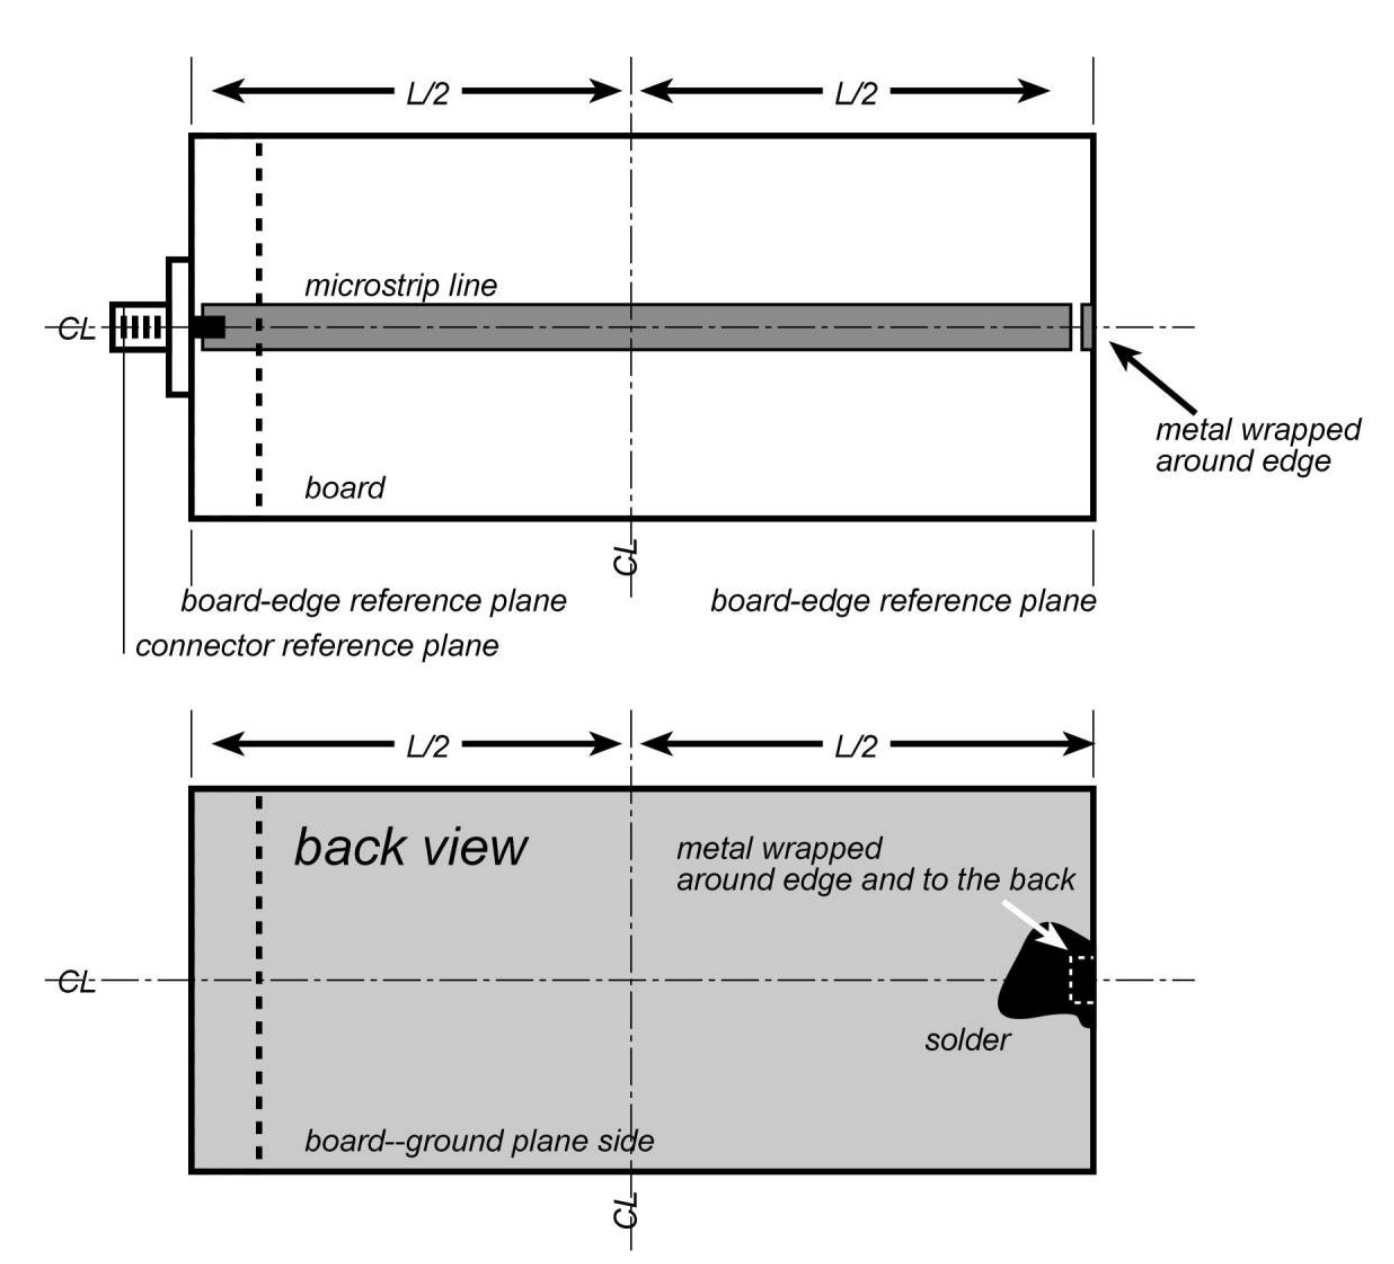
\includegraphics[width = 0.8\textwidth]{figures/Passive.jpg}
    \caption{Build mechanics for passive devices measurements}
\end{figure}

\begin{figure}[H]
    \centering
    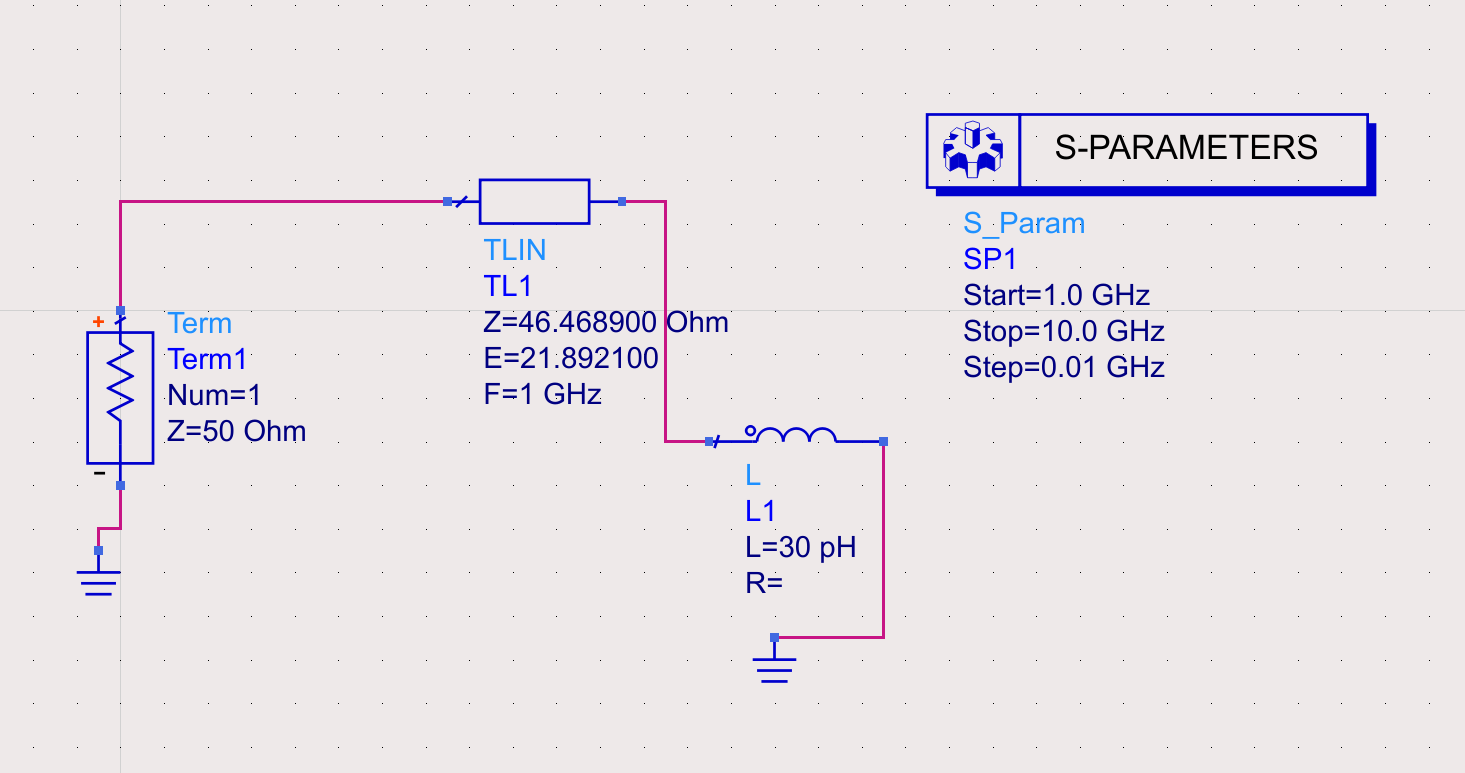
\includegraphics[width = 0.8\textwidth]{figures/schematic2.PNG}
    \caption{Simulation schematic for one of the passive devices}
    \label{fig:my_label}
\end{figure}












\section{Results}
\subsection{Transmission Line Measurement}
The results for 3mm, 5mm and 10mm transmission line measurements are plot as $S_{11}$ on the smith chart below.  

The results for 3mm, 5mm and 10 mm transmission line simulation are plots as $S_{11}$ below
\begin{figure}[h]
\centering
\begin{subfigure}{0.29\textwidth}
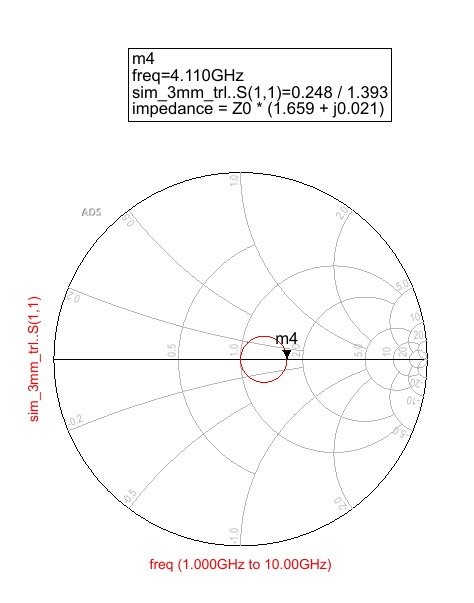
\includegraphics[width=1\linewidth,height = 5.5cm]{figures/tempplot/3mm_sim.jpg} 
\caption{3mm TL Simulation}
\label{fig:subim1}
\end{subfigure}
\begin{subfigure}{0.3\textwidth}
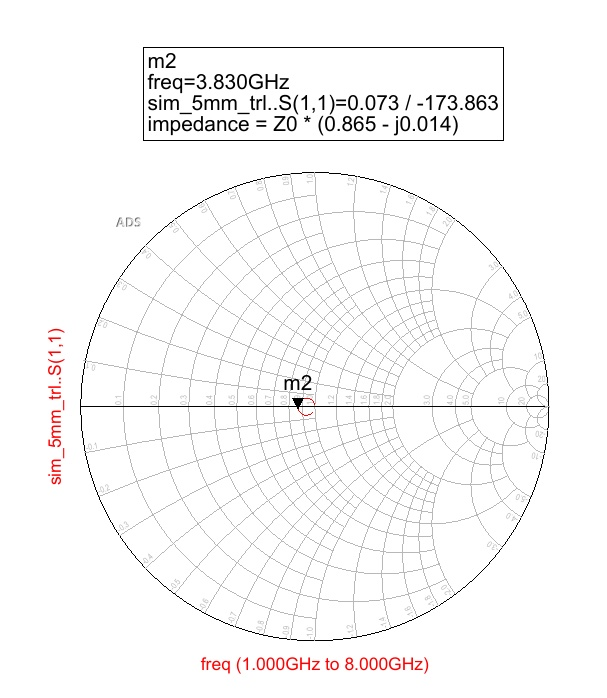
\includegraphics[width=1\linewidth,height = 5.5cm]{figures/tempplot/5mm_sim.jpg}
\caption{5mm Tl Simulation}
\label{fig:subim2}
\end{subfigure}
\begin{subfigure}{0.33\textwidth}
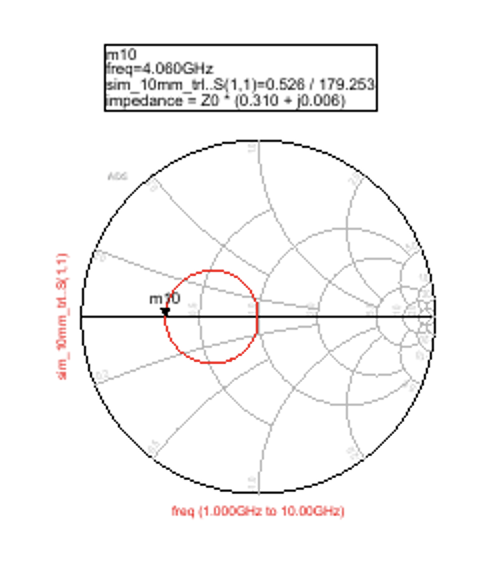
\includegraphics[width=1\linewidth, height = 5.5cm]{figures/tempplot/10mm_sim.png}
\caption{10mm Tl Simulation}
\label{fig:subim3}
\end{subfigure}
\end{figure}



\begin{flushleft}
In order to calculate the Characteristic Impedance, we use the formula below:
\end{flushleft}

\[Z_{in} =  \frac{{Z_0}^2}{Z_L}\]
Therefore:
\begin{equation}
    Z_0 = \sqrt{Z_{in}*Z_L} \quad \text{with} \quad Z_L = 50 \Omega
\end{equation}

\begin{flushleft}
With this function, we can calculate all the characteristic impedance from our measurement. To compute conveniently, we chose a marker on the middle line in the smith chart, thus meaning the capacitance and inductance can be negligible. The values of the impedance are listed in the table below. From the results we can observe that although the data is quite noisy, we still get reasonable impedance measurements which has a fairly low error compared to the theoretical values we get from the LineCalc. 
\end{flushleft}

\begin{center}
\begin{tabular}{||c c c c||} 
 \hline
 \quad & 3mm & 5mm & 10mm \\ [0.7ex] 
 \hline\hline
 LineCalc($\Omega$) & 64.41 & 46.47 & 27.86 \\ [0.7ex] 
 \hline
 Measurement($\Omega$) & 65.12 & 47.12 & 28.24 \\[0.7ex] 
 \hline
 Error(\%) & 1.10 & 1.39 & 1.38 \\[0.7ex] 
 \hline

\end{tabular}
\end{center}







In order to compute the phase velocity along the line, we refer back to the fundamental physical definition.
\begin{equation}
    v_{ph} = \frac{\omega}{k} = \frac{-l \omega}{\phi(\omega)}
\end{equation}
This statement may be evaluated to find a reasonable amount of agreement among the line widths tested.
Despite the noise in the measurements (especially at lower frequencies, due to effectively averaging over fewer samples,
we note an overall agreement among the traces to around $2.3 \cdot 10^8 \si{\meter\per\second}$, which is a notable but not fundamentally unreasonable error above theory.


\begin{figure}[H]
  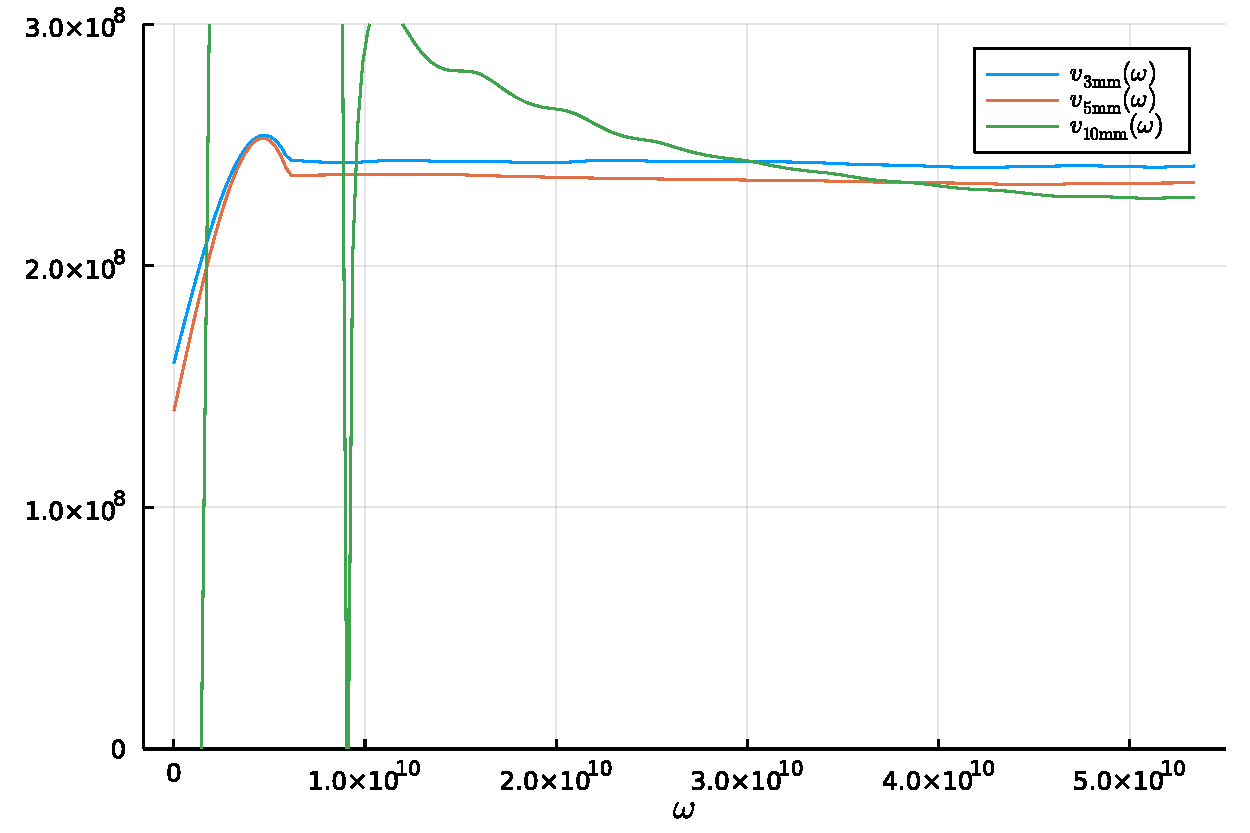
\includegraphics[width=0.8\textwidth]{figures/build/phase_vel.pdf}
  \caption{Effective phase velocity, measured for excitations at angular frequency $\omega$.}
  \label{fig:phasevel}
\end{figure}

\subsection{Passive Devices Measurement}

\begin{flushleft}
As mentioned above, we mentioned a 50 $\Omega$ 1/4-inch-long-leaded resistor a 50$\Omega$ very-short-leaded resistor, a 15 $\Omega$ chip resistor, a 100pF leaded capacitor, a 100pF chip capacitor, and a 30pH hand-made inductor. We will calculate the measured resistance for the resistor, the capacitance for the capacitor and inductance for the inductor. The formula is :
\end{flushleft}

\begin{equation}
    Z_{in} = R + jX 
    \quad \text{with Capacitor: } \quad X= \frac{1}{j\omega C}
    \quad \text{with Inductor: } \quad X= j \omega L
\end{equation}

\begin{flushleft}
Therefore we derive the formula for the measured load resistance, capacitance, and inductance as follows:
\end{flushleft}

\begin{equation}
 
      \quad \text{For Resistor: }\quad 
    Z_L = \frac{{Z_0}^2}{Z_{in}} \quad text{with Z_in is given as the impedance in the marker; Z_0 is calculated above} \quad 
    \quad \text{For Capacitance: }\quad 
    C = \frac{1}{j \omega X} \\
    \quad \text{For Inductance: }\quad
    L = \frac{X}{j \omega}

   
\end{equation}







\end{document}



